%%%%%%%%%%%%%%%%%%%%%%%%%%%%%%%%%%%%%%%%%%%%%%%%%%%%%%%%%%%%%%%%%%
%%%%%%%% ICML 2012 EXAMPLE LATEX SUBMISSION FILE %%%%%%%%%%%%%%%%%
%%%%%%%%%%%%%%%%%%%%%%%%%%%%%%%%%%%%%%%%%%%%%%%%%%%%%%%%%%%%%%%%%%

% Use the following line _only_ if you're still using LaTeX 2.09.
%\documentstyle[icml2012,epsf,natbib]{article}
% If you rely on Latex2e packages, like most moden people use this:
\documentclass{article}

% For figures
\usepackage{graphicx} % more modern
%\usepackage{epsfig} % less modern
\usepackage{subfigure}

% For citations
\usepackage{natbib}

% For algorithms
\usepackage{algorithm}
\usepackage{algorithmic}

% As of 2011, we use the hyperref package to produce hyperlinks in the
% resulting PDF.  If this breaks your system, please commend out the
% following usepackage line and replace \usepackage{icml2012} with
% \usepackage[nohyperref]{icml2012} above.
\usepackage{hyperref}

% Packages hyperref and algorithmic misbehave sometimes.  We can fix
% this with the following command.
\newcommand{\theHalgorithm}{\arabic{algorithm}}

% Employ the following version of the ``usepackage'' statement for
% submitting the draft version of the paper for review.  This will set
% the note in the first column to ``Under review.  Do not distribute.''
%\usepackage{icml2012}
% Employ this version of the ``usepackage'' statement after the paper has
% been accepted, when creating the final version.  This will set the
% note in the first column to ``Appearing in''
\usepackage[accepted]{icml2012}


% The \icmltitle you define below is probably too long as a header.
% Therefore, a short form for the running title is supplied here:
\icmltitlerunning{Weather Forecasting using Probabilistic Graphical Models}

\begin{document} 

\twocolumn[
\icmltitle{Weather Forecasting using Probabilistic Graphical Models}

% It is OKAY to include author information, even for blind
% submissions: the style file will automatically remove it for you
% unless you've provided the [accepted] option to the icml2012
% package.
\icmlauthor{Felipe Hernandez}{felipeh@andrew.cmu.edu}
\icmladdress{Depertment of Civil and Environmental Engineering, University of Pittsburgh}
\icmlauthor{Amos Ng}{ajng@andrew.cmu.edu}
\icmladdress{Language Technologies Institute, Carnegie Mellon University}

% You may provide any keywords that you 
% find helpful for describing your paper; these are used to populate 
% the "keywords" metadata in the PDF but will not be shown in the document
\icmlkeywords{boring formatting information, machine learning, ICML}

\vskip 0.3in
]

\begin{abstract} 
Weather prediction has usually involved running physical models of weather
phenomena in order to predict future conditions. In this project, instead of
focusing on the physics, we propose using probabilistic models based on
meteorological observations gathered by NASA to produce future weather
conditions.
\end{abstract} 

\section{Introduction}
\label{submission}

Weather forecasting is used for a broad range of purposes, ranging from personal
activity planning to large-scale economic decision-making to emergency
preparation and response. The availability and accuracy of forecasts thus have a
profound impact on human activities at many levels, both in measurable and
unmeasurable aspects.

However, predicting weather is a difficult research problem. Most often,
physically-based models with global and regional scales are used to forecast
future conditions. In this project, we will instead take a probabilistic machine
learning approach focused on a regional scale and predict atmospheric variables
at specific geographic locations.

The forecasts will be based on prior atmospheric states in the neighborhood of
the selected location. In particular, we will attempt to predict the probability
distributions of variables such as pressure, precipitation, and temperature
based on data recorded by NASA using assimilated land products.

\section{Related work} 
 
Researchers in the atmospheric sciences have investigated a variety of methods
for weather forecasting. Many subtle physical phenomena affect the weather at
any given time, including energy and mass transfer between the sun and different
layers of the atmosphere, ground, and ocean. Machine learning approaches have
been explored to construct simplified models based on atmospheric measurements,
but are not very popular among meteorologists.

Many of these techniques are tailored to fit the nature of the observations
available. Weather monitoring stations are the predominant data source,
providing point measurements with high accuracy and varying temporal resolution.
Artificial neural networks have proven to be effective in such cases for
forecasting rainfall amounts in the near future given a time series of
previously observed values \cite{maier2000}. More recent works have attempted to
combine NNs with other techniques to improve the performance of predictions. In
\cite{hong2008}, a recursive NN is trained using a support vector regression
together with a chaotic particle swarm optimizer. Other algorithms used in
weather forecasting include linear regression, discriminant analysis, logistic
regression \cite{applequist2002}.

Recently, meteorological observations from satellite and Doppler radar have
become widely available, providing ubiquitous coverage at the cost of decreased
precision. These sources of information add spatial dimensions to the
forecasting problem. For example, Fourier spectrum, structure function, and
moment-scale analyses are used to understand radar precipitation in
\cite{harris2007}. Forecasting models have also been created to take advantage
of interdependencies between atmospheric variables that are measured or
estimated using other models. Rain-gauge data and outputs from atmospheric
models are used for forecasting precipitation in \cite{kuligowski1998} and
\cite{ramirez2005}.

\section{Data collection}

As mentioned previously, there are multiple sources of meteorological
information available online. Usually these sources are provided by government
agencies such as NOAA and NASA, and have different levels of post-processing of
raw data from gauges, land radars, and satellites.

The North American Land Data Assimilation System (NLDAS), a service hosted by
the Goddard Earth Sciences Data and Information Services Center at NASA, is a
multi-variable source of information produced through the assimilation of land
measurements. We will focus mainly on this dataset due to both its relative high
precision and the multiple variables it reports: precipitation, atmospheric
pressure, humidity, temperature, wind speed, convective potential energy, and
radiation flux.

The NLDAS product provides hourly weather data for the US beginning in 1980.
Each sampled time in the data set includes the following values per cell in a
grid of resolution 1/8 of a degree in both latitude and longitude directions.
Figure~\ref{fig:example_rainfall} provides an illustration of one such hour-long
sample.


\begin{figure}[ht] \vskip 0.2in
\begin{center}
\centerline{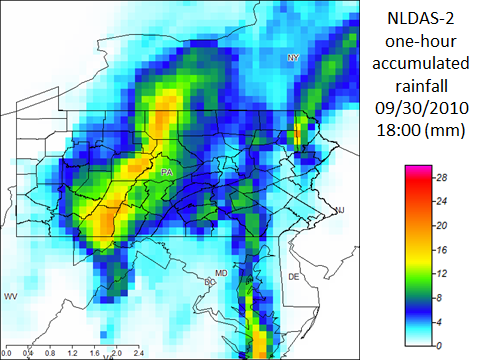
\includegraphics[bb=0 0 487 360,width=\columnwidth]{weather.png}}
\caption{This is one example of a rainfall image produced during a severe storm in Pennsylvania in 2010. Each cell in this image has a size of roughly 10 km $\times$ 10 km. More information on the NLDAS-2 data products can be found on the following URLs: \url{http://ldas.gsfc.nasa.gov/index.php} and \url{http://disc.sci.gsfc.nasa.gov/hydrology/data-holdings}.}
\label{fig:example_rainfall}
\end{center}
\vskip -0.2in
\end{figure}

Thus far we have downloaded the data from the above links, over the range of a few months. We put the data into a database for efficient storage and retrieval. We then used the Graphical LASSO (GLASSO) training algorithm to obtain the precision matrix for relations between the various variables in the data. The results, shown in Table~\ref{tab:precision}, indicate that precipitation is only directly linked to sufrace pressure, which in turn is linked with the rest of the variables.

\begin{table*}[t]
\begin{tabular}{ p{1cm} p{2cm} p{2cm} p{2cm} p{2cm} p{2cm} p{2cm} p{2cm}}
& Precipitation & Available potential energy & LW radiation & SW radiation & Surface pressure & Temperature 2 m & Wind speed\\
\hline
P   & 1.978e-02 & 0.000e+00 & 0.000e+00 & 0.000e+00 & 1.956e-06 & 0.000e+00 & 0.000e+00\\
APE &0.000e+00 & 2.196e-05 &-3.935e-05 &-2.069e-06 & 8.472e-07 &-9.129e-05 &-3.384e-05\\
LW R&0.000e+00 &-3.935e-05 & 7.906e-04 &-1.638e-05 & 4.472e-06 &-4.096e-04 & 0.000e+00\\
SW R&0.000e+00 &-2.069e-06 &-1.638e-05 & 2.341e-05 &-1.041e-06 &-1.383e-04 &-1.719e-05\\
SP  &1.956e-06 & 8.472e-07 & 4.472e-06 &-1.041e-06 & 4.021e-06 & 0.000e+00 & 1.189e-05\\
T   &0.000e+00 &-9.129e-05 &-4.096e-04 &-1.383e-04 & 0.000e+00 & 1.440e-02 & 0.000e+00\\
WS  &0.000e+00 &-3.384e-05 & 0.000e+00 &-1.719e-05 & 1.189e-05 & 0.000e+00 & 1.880e-02\\
\end{tabular}
\caption{The precision matrix obtained from results thus far, using a GLASSO regularization parameter of $\rho = 50$. Log-likelihood for the data given this precision matrix stands at $-376$. Note that all variables (``percentage convective precipitation,'' ``potential evaporation,'' and ``specific humidity'') that had zero covariance with all variables other than itself, are not included in this table.}
\label{tab:precision}
\end{table*}

\section{Proposed method}

\section{Activity plan}

We plan to use different probabilistic graphical models to try to determine the
probability distributions of weather variables maps given the observed values
from previous time steps. We will first use variable discretization so that
discrete models can be used. Afterwards, we will attempt using models that are
able to handle continuous variables.

To establish a baseline approach, we will first use simple graph
representations, such as Na�ve Bayes networks. Later, we will attempt to use
models with more complex topologies that take into account the interdependencies
of variables.

Some of the activities that we will perform include
\begin{enumerate}
\item Selection of the dataset and the study area
\item Data download and pre-processing
\item Variable discretization strategy
\item Na\"\i ve Bayes formulation
\item Review of probabilistic graphical models for continuous variables
\end{enumerate}

\nocite{nasseri2008}

\bibliography{bibliography}
%\bibliographystyle{icml2012}

\end{document} 


% This document was modified from the file originally made available by
% Pat Langley and Andrea Danyluk for ICML-2K. This version was
% created by Lise Getoor and Tobias Scheffer, it was slightly modified  
% from the 2010 version by Thorsten Joachims & Johannes Fuernkranz, 
% slightly modified from the 2009 version by Kiri Wagstaff and 
% Sam Roweis's 2008 version, which is slightly modified from 
% Prasad Tadepalli's 2007 version which is a lightly 
% changed version of the previous year's version by Andrew Moore, 
% which was in turn edited from those of Kristian Kersting and 
% Codrina Lauth. Alex Smola contributed to the algorithmic style files.  


